\documentclass{article}
\usepackage[preprint]{ge2340_project}
\usepackage[utf8]{inputenc}
\usepackage[T1]{fontenc}
\usepackage{url}
\usepackage{booktabs}
\usepackage{amsmath,amssymb}
\usepackage{graphicx}
\usepackage{microtype}
\usepackage{xcolor}
\usepackage{float}
\usepackage{hyperref}
\setcitestyle{numbers,square}
\hypersetup{colorlinks=true,linkcolor=blue,citecolor=blue,urlcolor=blue,
  pdftitle={Phase 2: Course Registration Helper for Balanced Workloads},pdfauthor={}}
\urlstyle{same}
\title{Phase 2: AI Project Report\\
\large Course Registration Helper for Balanced Workloads}
\author{}

\begin{document}
\maketitle

\section{Introduction \& Problem Recap}
We created the Course Registration Helper to help City University of Hong Kong students turn academic requirements and personal interests into a coherent study plan. Supporting Computing Mathematics (CM) and Computer Science (CS), our system connects programme rules, GE choices and timetables. Students can select a stream and adjust priorities for background suitability, difficulty and workload.

Our design combines a fine-tuned language model with mathematical optimisation. The model interprets course information and proposes structured recommendations; source checks and an optimiser turn them into a constrained plan. This lets us personalise recommendations while respecting programme eligibility and academic dependencies.

We extend the original workload-balancing proposal with rewards for graduation progress, preparation and stream completion. In our initial source-conditioned evaluation, fine-tuning increased exact-answer performance from 20.0\% to 93.3\%. Controlled experiments confirm that penalty settings change elective choices and prior study changes configured rewards, establishing an explainable foundation for personalised planning.

\section{Data Collection \& Methodology}
\textbf{A programme-specific knowledge base.} We assembled the student handbook, CM degree path and course list, CS major requirements and suggested plan, GE information, and saved Semester A/B timetable pages\citep{cityu-programmes}. We preserve source cohorts and academic years: the CM path concerns the 2025 intake, its designated course list is historical, and CS requirements and its suggested plan cover different academic-year contexts. These distinctions remain visible when rules need confirmation.

\begin{table}[H]
\centering\small
\caption{Coverage of our programme and timetable collection.}
\begin{tabular}{p{3.85in}r}
\toprule
Knowledge-base component & Coverage\\
\midrule
Distinct timetable files after duplicate removal & 93\\
Course--term--programme records & 86\\
Sections matching the encoded major restrictions & 128\\
CM / CS document-listed course codes & 85 / 73\\
GE codes in the original import & 64\\
Files excluded because meeting times were unrecognised & 7\\
\bottomrule
\end{tabular}
\label{tab:data}
\end{table}

\textbf{Turning documents into usable rules.} We extracted meeting days/times, prerequisites, exclusions and restrictions, removed duplicates and retained sources. ``ONLY FOR CM'' is an explicit major restriction. Candidates must appear in the student's designated programme document or the verified GE collection, then satisfy further eligibility checks. Entries with missing times are excluded from verified timetable planning. GE2340 was separately verified for the AI-interest examples.

\newpage
\textbf{Training and evaluation design.} Our initial programme dataset contains 485 training, 24 validation and 30 test examples combining curriculum/timetable extraction with synthetic stream-policy answers. Its before/after comparison uses 15 preselected queries across membership, sections, course rules, source extraction and stream reasoning. The CM finance-background update uses 244 training and 32 validation examples, plus 20 held-out profile/candidate combinations. Both comparisons use the same base-loading protocol for each pair. Shared source facts and synthetic policies mean these are familiar-evidence tests, rather than unseen-cohort evaluations.

We complement this comparison with controlled penalty experiments, dependency interventions and 20 fictional student profiles. Fictional transcripts let us vary academic histories without using real student records. Workload and preparation scores are transparent, editable estimates; they have not yet been validated against student study-time or assessment outcomes. Some syllabus evidence comes from indexed official excerpts, including historical sources, where direct access was unavailable.

\section{Implementation Details}
\textbf{From student profile to explained recommendation.} Our pipeline combines course evidence, the student's passed courses and their preferences. The language model returns structured proposals, which we check against exact local rules. The planner then evaluates eligible options and explains the selected route, reward contributions and unresolved requirements (Figure~\ref{fig:workflow}). A rejected model answer can be replaced by source lookup or exact policy calculation, with that intervention recorded separately.

\begin{figure}[H]
\centering
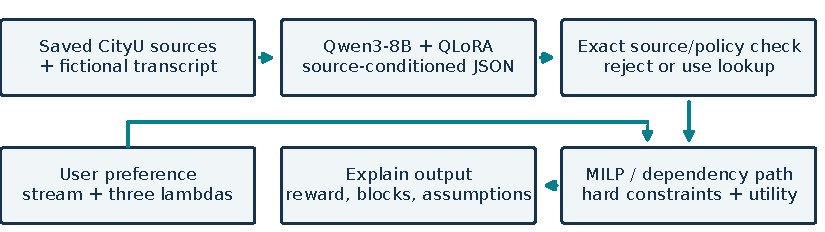
\includegraphics[width=\linewidth]{figures/workflow.pdf}
\caption{Our planning pipeline connects course evidence and student preferences to validated recommendations and an explanation of the result.}
\label{fig:workflow}
\end{figure}

\textbf{Efficient model adaptation.} We fine-tuned Qwen3-8B\citep{qwen} using rank-8 QLoRA\citep{qlora}, with a frozen four-bit base and BF16 computation. This adapts approximately 21.8 million parameters on a single RTX 5090. The finance-background fine-tune completed two epochs in approximately 5.5 minutes, with 7.37 GiB peak allocated GPU memory. Validation loss decreased from 0.13366 to 0.00135. We retained the first epoch because its validation result was better than the second.

We use supervised cross-entropy to teach structured responses. The planner's academic-profit objective is a separate optimisation function: training teaches the model to express the relevant information, while the optimiser decides which feasible course combination best fits the student's preferences. This separation makes preference changes immediate without requiring retraining.

\textbf{Student control.} Our local interface accepts a transcript profile, a desired stream, a stream-priority weight and three penalty weights. It provides course lookup, stream proposals, dependency paths and semester planning. The optimiser uses SciPy's mixed-integer linear programming interface\citep{scipy}. We retain experiment inputs, outputs and policy decisions so recommendations can be traced back to the evidence\citep{runs}.

\newpage
\textbf{An objective that rewards meaningful progress.} Let $s$ describe the student's completed courses, covered GE areas, year, credit progress and selected stream. For a feasible course set $X$, we maximise
\begin{align}
U(X,s)={}&\sum_{c\in X}\bigl[g_c(s)+p_c(s)+h_c(s)+q_c(s)\nonumber\\
&\quad-\lambda_b b_c(s)-\lambda_d d_c(s)-\lambda_w w_c(s)\bigr]
+R_{\mathrm{stream}}(X,s)-O(X,s). \label{eq:utility}
\end{align}
The positive terms reward base course value $g$, preparation $p$, graduation priorities $h$, prerequisite bridges $q$ and progress towards one selected stream $R_{\mathrm{stream}}$. The three non-negative weights $\lambda_b,\lambda_d,\lambda_w$ control penalties for background mismatch, difficulty and workload. Profit is expressed in academic-utility points. Minimising the planner's loss is equivalent to minimising $-U$.

\textbf{Personalisation across a degree.} A course normally has base profit 3. If a student has already covered its GE area, another distributional GE in that area receives only 0.3 base profit, encouraging breadth. A selected stream earns 2 points per new distinct requirement slot and a one-time 6-point completion reward. Students can adjust the stream multiplier from 0 to 10; an explicit choice normally uses weight 3. GE2260 can indicate finance interest, while GE2340 can indicate CS AI interest. The student's explicit stream choice takes precedence, and a GE preference never substitutes for a stream course or a formal prerequisite.

We account for both immediate progress and the next step in a course chain. For example, a prerequisite bridge can receive extra reward because it opens access to a preferred stream. Stream slots and completion rewards are counted once, including when several alternatives are selected together. In four-year simulations, the student's state is updated after each semester, allowing later decisions to reflect earlier choices.

Our overload penalty supports a lighter final year:
\begin{equation}
O(X,s)=\mathbf{1}_{\{\mathrm{year}=4\}}\,0.25\,[\max(0,C(X)-12)]^2,
\end{equation}
where $C(X)$ is semester credits. The penalty is zero in Years 1--3 and for at most 12 credits in Year 4; it increases to 2.25 at 15 credits and 9 at 18 credits. This encourages manageable final-year choices without penalising the standard earlier-year load.

\textbf{Background-focused CM planning.} For CM students, our planner allows an assumed prerequisite waiver for the listed EF and CS courses. Missing those formal passes adds no extra penalty. We instead assess finance preparation: background mismatch is 0.45 without evidence, 0.15 for introductory study and 0.05 for advanced passed study. Passed finance GEs or an explicit study declaration can supply introductory evidence; failed/in-progress courses do not. This is an advisory assumption, not verified university waiver approval.

\textbf{Academic requirements remain binding.} Programme membership, exclusions, required courses, credit bounds, section restrictions and timetable conflicts still apply. Mathematics and non-CM prerequisites remain enforced. Defaults require 5--6 courses in Years 1--3, with at most 18 credits; the Year 4 minimum is waived. Distributional GE is capped at one per semester, excluding compulsory language/development courses. Our CM degree simulation targets at least 122 credits, four distributional GEs spanning all three areas and at least 20 elective mathematics credits outside core/capstone study. The source's 122-credit threshold also meets the requested 121-credit minimum.

Unknown component linkage or teaching weeks is flagged. Hypothetical timetable examples explicitly state their assumptions, and dependency layers describe academic order rather than guaranteed future semester offerings. These boundaries help students distinguish a useful planning route from confirmed registration availability.

\newpage
\section{Results \& Evaluation}
\textbf{Stronger understanding of programme information.} Our initial 15-query source-conditioned test improved from 3 correct answers before fine-tuning to 14 afterwards. Membership, section, course-rule and source-extraction tasks each reached 3/3; stream reasoning reached 2/3. This supports the value of adapting the model to the structure of our course documents. The remaining stream-counting error also demonstrates the value of exact validation. A corrective training trial introduced a different error and was not selected, showing why we retain validation and checkpoint comparison in our development process.

\textbf{Learning the CM background rule.} Follow-up training improved exact answers from 0/20 to 18/20 on the new policy test; existing-task checks remained at 5/6. All six default-profile diagnostics passed. Two waiver-applicability errors were rejected by validation. These familiar-policy tests evaluate the configured rule, not real student outcomes.

\textbf{Three penalties give students meaningful control.} We tested six penalty settings on matched CM and CS fixtures. Four required three-credit courses, three alternative electives, scores and synthetic times remain fixed; only the weights change. Each resulting optimum was independently checked by enumerating the three alternatives.

\begin{table}[H]
\centering\small
\caption{Changing the three penalties changes the preferred elective. Each setting was tested separately for CM and CS with matched synthetic scores.}
\begin{tabular}{cccp{1.05in}p{1.05in}r}
\toprule
$\lambda_b$ & $\lambda_d$ & $\lambda_w$ & CM elective & CS elective & Net utility\\
\midrule
1 & 1 & 1 & MA3521 & CS4486 & 17.25\\
20 & 1 & 1 & MA3521 & CS4486 & 1.10\\
1 & 20 & 1 & MA3523 & CS3483 & $-5.90$\\
1 & 1 & 20 & MA3525 & CS3402 & $-5.75$\\
0 & 12 & 1 & MA3523 & CS3483 & 2.85\\
12 & 12 & 1 & MA3521 & CS4486 & $-8.05$\\
\bottomrule
\end{tabular}
\label{tab:lambda}
\end{table}

A stronger difficulty penalty selects MA3523/CS3483, while a stronger workload penalty selects MA3525/CS3402. A larger background penalty can change utility without changing the chosen course. All 12 constructed optima pass verification. Negative utility reflects binding study requirements under a demanding preference setting; values across different weight settings are not directly comparable measures of educational quality.

\textbf{Dependency experiment: how earlier study changes a reward.} We designed 12 paired interventions to isolate individual dependencies. Year, base profit, score vector and penalty weights remain fixed; credit-progress and overload effects are excluded. Table~\ref{tab:dependency} summarises the observed changes. All 12 match their predeclared policy effects.

\begin{table}[H]
\centering\small
\caption{Dependency effects with other utility components held fixed. Deltas are configured utility points. A prerequisite can unlock a course without increasing its numeric reward.}
\begin{tabular}{p{2.2in}p{0.65in}p{2.15in}}
\toprule
Changed history or preference & Target & Observed effect\\
\midrule
Pass MA2508 & MA3515 & Preparation reward $+0.20$\\
Pass MA2509 & GE2134 & Preparation reward $+0.15$\\
Replace Area-2 GE with Area-1 GE & GE1113 & Same-area base reward $-2.70$\\
Pass GE2260; finance selected & MA3521 & Stream reward $+4.00$\\
Pass GE2260; explicit Enriched choice & MA3521 & No reward change\\
Pass CS3481 & CS4487 & Prerequisite unlocked; reward unchanged\\
Pass CS4480; CS3481 already passed & CS4487 & Final-slot completion reward $+6.00$\\
Pass unrelated GE1305 & MA3521 & No reward change\\
Duplicate a passed MA2509 ID & GE2134 & No repeated preparation reward\\
Pass GE2260; finance bridge pending & MA2510 & Bridge reward $+2.00$\\
Pass GE2260; finance weight already 3 & MA3521 & No second preference multiplier\\
Pass MA2503; conceptual finance link & EF3320 & No preparation bonus from this link\\
\bottomrule
\end{tabular}
\label{tab:dependency}
\end{table}

\newpage
\textbf{Recognising a complete course chain.} We also tested an interaction in the Software Engineering and Project Management stream. The target CS4348 earns 2 stream points with neither CS3346 nor CS3356 passed, or with either one passed alone. With both passed, CS4348 becomes the final requirement and earns 8 points. The interaction $8-2-2+2=6$ correctly isolates the completion reward. All four model queries reproduce the expected policy answers (Figure~\ref{fig:interaction}). These are computational rule tests; source-date and offering restrictions still apply.

\begin{figure}[H]
\centering
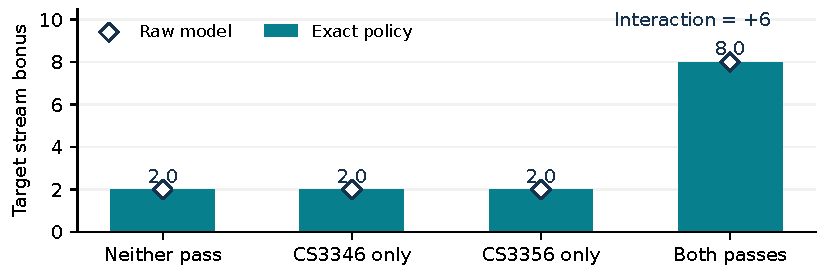
\includegraphics[width=\linewidth]{figures/stream_interaction.pdf}
\caption{Our model reproduces the stream-completion threshold in all four controlled cases. The additional six points reward finishing the chain.}
\label{fig:interaction}
\end{figure}

Grade controls reinforce this behaviour: a passed MA2509 receives its preparation benefit, while failed, in-progress and withdrawn records do not. Prerequisite-OR checks also recognise that either qualifying alternative is sufficient. These results validate our configured mechanisms; measured workload or learning benefits require a student study. An end-to-end schedule intervention remains future work, because a reward change does not necessarily change the best feasible timetable.

\textbf{Personalised paths across 20 student profiles.} We generated ten CM and ten CS fictional profiles with taught core completed, random GE histories and balanced desired-stream choices. With the CM waiver rule, our path checker produces 11 academic dependency paths, five advisory paths assuming the waiver and four provisional paths requiring further rule confirmation. Representative outputs appear in Table~\ref{tab:examples}. Capstones, internships and future offerings are not assumed satisfied.

\begin{table}[H]
\centering\small
\caption{Examples of the paths and obstacles our helper explains. Arrows indicate academic dependency order.}
\begin{tabular}{p{1.4in}p{2.2in}p{1.4in}}
\toprule
Student preference & Recommended route or identified obstacle & Planning result\\
\midrule
CM: Enriched Mathematics & MA3523, MA4542, MA4545 and MA4546 & Academic path\\
CS: Artificial Intelligence & CS3383 + CS4486 $\rightarrow$ CS4487 & Academic path\\
CS: Data Science & CS3402 + CS3481 $\rightarrow$ CS4480 + CS4487 & Bridge courses needed\\
CM: Financial Mathematics & {\raggedright MA3521, MA4529 + two of MA4537, EF3320 or EF4821\par} & Waiver assumed\\
\bottomrule
\end{tabular}
\label{tab:examples}
\end{table}

Before the finance-focused update, the model passed exact stream-policy validation in 10/20 of these profiles: 0/10 CM and 10/10 CS. Rejected answers used exact policy outputs. This historical result identifies the reasoning gap that motivated further training; the updated path counts above come from the revised policy checker.

The finance examples now prioritise relevant study rather than missing EF bridge passes. We retain the published prerequisite and exclusion evidence\citep{cityu-finance}, while the CM planning waiver removes prerequisite-only blocks. Actual offerings remain separate: the saved EF snapshots contain no matching CM sections. The helper therefore explains an advisory route without inventing a registerable section.

\newpage
\section{Discussion}
Our main contribution is a planner that makes the relationship between student preference and academic feasibility explicit. A desired stream shapes the reward, completed courses change the value of the next step, and the three penalties let students express their priorities. Source checks keep these preferences connected to programme requirements. In one document-filtered CM four-year simulation, the plan reaches 124 credits and completes a stream under the encoded requirements. A separate CM Semester A example is correctly reported as infeasible under the five-course minimum, demonstrating that the planner can expose a constraint problem rather than hide it.

During development, we found that reliable planning depended as much on organising course evidence as on fine-tuning. Saved pages made collection reproducible when authenticated pages or security challenges restricted access. Duplicate removal, explicit major matching and source-year tracking prevented misleading combinations of otherwise plausible course information. These practical lessons shaped our emphasis on traceable recommendations.

The current evidence supports the model's usefulness for interpreting supplied information and exploring configured preferences. It does not yet establish real workload reduction or generalisation to new cohorts. The small training evaluation shares source documents, the profile studies use fictional histories, and later CM examples expose a clear reasoning gap. We therefore evaluate model answers separately from policy corrections and retain source uncertainty in the final explanation. CS experiments cover paths and semesters, rather than a verified full-degree audit.

Our next step is to combine current, cohort-consistent rules and confirmed section bundles with lecturer-reviewed workload evidence. Assessment-week deadlines and consented student study-time data would let us test the original goal of balancing workload across a semester. Independent documents, paired schedule experiments and new student cohorts should measure recommendation quality beyond policy agreement. Students should remain able to override inferred GE interests; any real-transcript study would use consent, minimal retention and clear deletion controls.

\section{Conclusion}
We built a personalised course-planning system that combines fine-tuned language understanding, source-based validation and mathematical optimisation. Students can explore streams, adjust three penalty weights and see how earlier study affects the value of later courses. Our initial test improves from 20.0\% to 93.3\%, and controlled experiments verify penalty sensitivity and dependency rewards. Later profile failures identify where model reasoning still needs improvement. With traceable rules and explicit feasibility checks, our helper provides a practical foundation for more informed course choices and future evidence-based workload planning.

\begin{thebibliography}{9}
\small
\bibitem[Yang et~al.(2025)]{qwen}
A. Yang et al., ``Qwen3 Technical Report,'' arXiv:2505.09388, 2025.
\url{https://arxiv.org/abs/2505.09388}. Model: \url{https://huggingface.co/Qwen/Qwen3-8B}.

\bibitem[Dettmers et~al.(2023)]{qlora}
T. Dettmers, A. Pagnoni, A. Holtzman and L. Zettlemoyer, ``QLoRA: Efficient Finetuning of Quantized LLMs,'' 2023. \url{https://arxiv.org/abs/2305.14314}.

\bibitem[SciPy contributors()]{scipy}
SciPy contributors, ``\texttt{scipy.optimize.milp},'' official documentation.
\url{https://docs.scipy.org/doc/scipy/reference/generated/scipy.optimize.milp.html}.

\bibitem[CityUHK(2022--2026)]{cityu-programmes}
CityUHK, supplied \emph{Student Handbook 2026--27}, CM 2025-entry normative path and designated course list; CS major requirements (2026/27) and 2025-cohort normative plan; saved GE and Semester A/B timetable pages.

\bibitem[CityUHK()]{cityu-finance}
CityUHK, course catalogue and saved rule evidence for GE2260, CB3410 and EF prerequisite chains. \url{https://www.cityu.edu.hk/catalogue/ug/current/course/GE2260.htm}; \url{https://www.cityu.edu.hk/catalogue/ug/current/course/EF3320.htm}. Historical conflicts remain flagged.

\bibitem[Project experiment records(2026)]{runs}
Course Registration Helper experiment records, 21 November 2026: programme training/evaluation, penalty sensitivity, desired-stream profiles and dependency interventions. Inputs, outputs and source hashes are retained in the accompanying project evidence.
\end{thebibliography}
\end{document}
